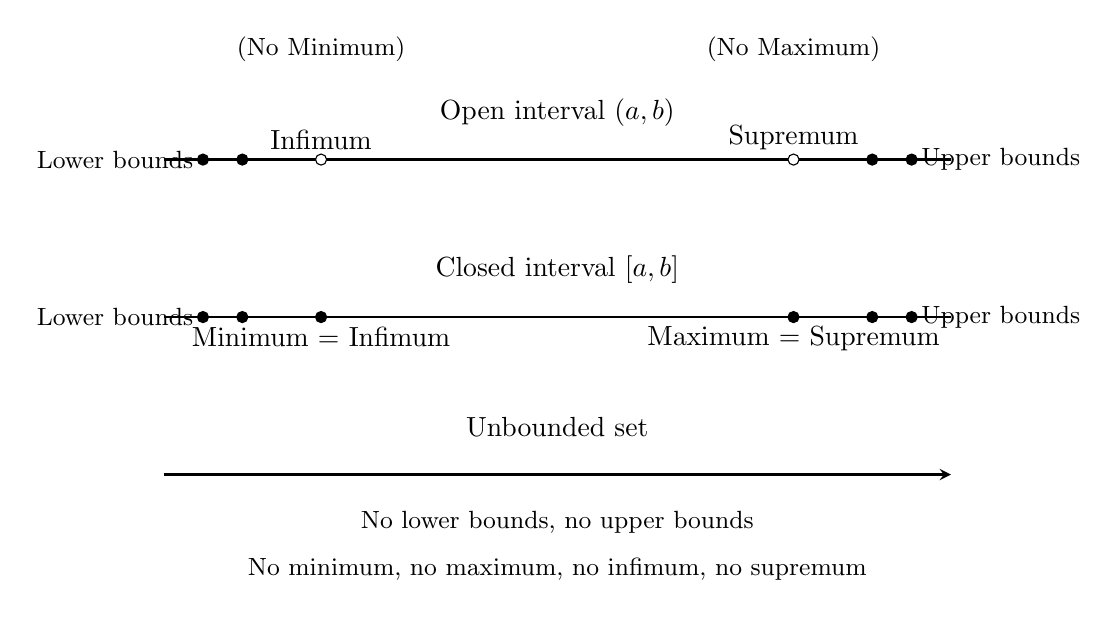
\begin{tikzpicture}[x=1cm,y=1cm,>=stealth]

% =====================
% OPEN INTERVAL (a,b)
% =====================
\draw[thick] (-5,3) -- (5,3);
\draw[fill=white] (-3,3) circle (2pt);
\draw[fill=white] (3,3) circle (2pt);

\node at (0,3.6) {Open interval $(a,b)$};

% Infimum / Supremum
\node[above] at (-3,3) {Infimum};
\node[above] at (3,3) {Supremum};
\node at (-3,4.4) {\small (No Minimum)};
\node at (3,4.4) {\small (No Maximum)};

% Lower bounds
\draw[fill] (-4.5,3) circle (2pt);
\draw[fill] (-4,3) circle (2pt);
\node[left] at (-4.5,3) {\small Lower bounds};

% Upper bounds
\draw[fill] (4,3) circle (2pt);
\draw[fill] (4.5,3) circle (2pt);
\node[right] at (4.5,3) {\small Upper bounds};

% =====================
% CLOSED INTERVAL [a,b]
% =====================
\draw[thick] (-5,1) -- (5,1);
\draw[fill] (-3,1) circle (2pt);
\draw[fill] (3,1) circle (2pt);

\node at (0,1.6) {Closed interval $[a,b]$};

% Min / Max
\node[below] at (-3,1) {Minimum = Infimum};
\node[below] at (3,1) {Maximum = Supremum};

% Lower bounds
\draw[fill] (-4.5,1) circle (2pt);
\draw[fill] (-4,1) circle (2pt);
\node[left] at (-4.5,1) {\small Lower bounds};

% Upper bounds
\draw[fill] (4,1) circle (2pt);
\draw[fill] (4.5,1) circle (2pt);
\node[right] at (4.5,1) {\small Upper bounds};

% =====================
% UNBOUNDED SET
% =====================
\draw[thick,->] (-5,-1) -- (5,-1);

\node at (0,-0.4) {Unbounded set};

\node at (0,-1.6)
{\small No lower bounds, no upper bounds};

\node at (0,-2.2)
{\small No minimum, no maximum, no infimum, no supremum};
\end{tikzpicture}